% Options for packages loaded elsewhere
\PassOptionsToPackage{unicode}{hyperref}
\PassOptionsToPackage{hyphens}{url}
%
\documentclass[
]{article}
\usepackage{amsmath,amssymb}
\usepackage{lmodern}
\usepackage{iftex}
\ifPDFTeX
  \usepackage[T1]{fontenc}
  \usepackage[utf8]{inputenc}
  \usepackage{textcomp} % provide euro and other symbols
\else % if luatex or xetex
  \usepackage{unicode-math}
  \defaultfontfeatures{Scale=MatchLowercase}
  \defaultfontfeatures[\rmfamily]{Ligatures=TeX,Scale=1}
\fi
% Use upquote if available, for straight quotes in verbatim environments
\IfFileExists{upquote.sty}{\usepackage{upquote}}{}
\IfFileExists{microtype.sty}{% use microtype if available
  \usepackage[]{microtype}
  \UseMicrotypeSet[protrusion]{basicmath} % disable protrusion for tt fonts
}{}
\makeatletter
\@ifundefined{KOMAClassName}{% if non-KOMA class
  \IfFileExists{parskip.sty}{%
    \usepackage{parskip}
  }{% else
    \setlength{\parindent}{0pt}
    \setlength{\parskip}{6pt plus 2pt minus 1pt}}
}{% if KOMA class
  \KOMAoptions{parskip=half}}
\makeatother
\usepackage{xcolor}
\usepackage{graphicx}
\makeatletter
\def\maxwidth{\ifdim\Gin@nat@width>\linewidth\linewidth\else\Gin@nat@width\fi}
\def\maxheight{\ifdim\Gin@nat@height>\textheight\textheight\else\Gin@nat@height\fi}
\makeatother
% Scale images if necessary, so that they will not overflow the page
% margins by default, and it is still possible to overwrite the defaults
% using explicit options in \includegraphics[width, height, ...]{}
\setkeys{Gin}{width=\maxwidth,height=\maxheight,keepaspectratio}
% Set default figure placement to htbp
\makeatletter
\def\fps@figure{htbp}
\makeatother
\setlength{\emergencystretch}{3em} % prevent overfull lines
\providecommand{\tightlist}{%
  \setlength{\itemsep}{0pt}\setlength{\parskip}{0pt}}
\setcounter{secnumdepth}{-\maxdimen} % remove section numbering
\ifLuaTeX
  \usepackage{selnolig}  % disable illegal ligatures
\fi
\IfFileExists{bookmark.sty}{\usepackage{bookmark}}{\usepackage{hyperref}}
\IfFileExists{xurl.sty}{\usepackage{xurl}}{} % add URL line breaks if available
\urlstyle{same} % disable monospaced font for URLs
\hypersetup{
  hidelinks,
  pdfcreator={LaTeX via pandoc}}

\author{}
\date{}

\begin{document}

\textbf{Simularea variațiilor Hill Climbing și Simulated Annealing
pentru optimizarea funcțiilor test (Sphere/De Jong, Rastrigin, Schwefel,
Michalewicz)}\\
\textbf{Autor:} Negură Teodor Alexandru

\hypertarget{rezumat-abstract}{%
\subsection{Rezumat (Abstract)}\label{rezumat-abstract}}

\begin{itemize}
\tightlist
\item
  Problema Studiata : Gasirea minimului global pe domeniul celor 4
  functii matematice
\item
  Metode: Algoritmul Hill Climbing(First Improvement/Best Improvement
  /Worst Improvement), Simulated Annealing hibridizat cu Best
  Improvement .
\item
  Setări experimentale esențiale: D$\in$\{5,10,30,100\}, N=50
  rulari/configuratie Functie-Variatie\_Alg-Dimensiune, buget
  E=\{50,100,250\}*10000*D evaluări, $\delta$ definit pentru precizie de 5
  zecimale si răcire geometrică in cadrul SA.
\item
  Rezultate cheie
\item
\item
  Concluzie si o direcție viitoare.
\end{itemize}

\hypertarget{introducere}{%
\subsection{1. Introducere}\label{introducere}}

\textbf{1.1 Context \& motivație:} Optimizare cu peisaje multi‑modale,
cost evaluare,\\
\textbf{1.2 Problema.} Minimizare celor 4 functii matematice (f(x)) , pe
domeniu ({[}a,b{]}\^{}D).\\
\textbf{1.3 Contribuții.} (a) Protocol experimental echitabil (buget infinit
D), (b) analiză parametrică $\delta$, T0, $\delta$, L, (c) hibrid SA→BI și comparație
cu HC clasice.\\
\textbf{1.4 Structura raportului.}

\begin{quote}
\textbf{Checklist secțiune:} clarifică obiectivul (minimizare),
definește ``fitness'', spune pe ce dimensiuni lucrezi și de ce,
precizează criteriul de comparație (buget fix sau până la $\epsilon$).
\end{quote}

\hypertarget{fundamente-funcux21bii-test}{%
\subsection{\texorpdfstring{2. Fundamente \& Funcții test
}{2. Fundamente \& Funcții test }}\label{fundamente-funcux21bii-test}}

\textbf{2.1 Notări și termeni.}

"\textbf{H.C.}" - HillClimbing

"\textbf{S.A.}" - Simulated Annealing

"\textbf{Fitness}" - valoarea functiei matematice f in punctul x de
coorodnate {[}x1,x2,...,xn{]}.Cu alte cuvinte , fitnesul functiei f , in
punctul x cu coordonatele expuse mai devreme si variabile in functie de
dimensiunea D = f(x1) + f(x2) + ... + f(xn);

``\textbf{Vecin}'' - adunarea sau scaderea valorii delta dintr-o singura
coordonata a unui punct aleatoriu , indidfrent de lungime.

``\textbf{Delta}'' = valoare ajutatoare pt calculaul vecinilor , =
0.00001

\textbf{``Dimensiune}''= lungimea sirului de coordonate a unui punct
aleatoriu x. avem x{[}x1,x2,...,xn{]}, in Dimensiunea D , considera n ca
fiind egal cu D.

``\textbf{Functie Unimodala}'' = un singur optim global și niciun alt
optim local.

``\textbf{Functie Multimodala}'' = un optim global, dar și mai mulți
optimi locali.

\textbf{2.2 Domenii \& formule:}

\textbf{De Jong1(continua,grafic convex si unimodala):}

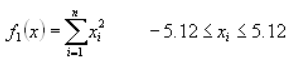
\includegraphics[width=3.05251in,height=0.6876in]{vertopal_3cc9e404d6084a9aa4179e4b559e5481/media/image1.png}

\textbf{Schwefel(multimodala):}

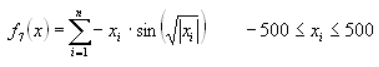
\includegraphics[width=3.94847in,height=0.69801in]{vertopal_3cc9e404d6084a9aa4179e4b559e5481/media/image2.png}\\
\textbf{Rastrigin(multe minime locale):}

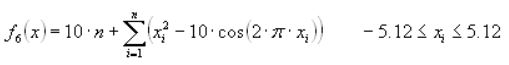
\includegraphics[width=5.30282in,height=0.67718in]{vertopal_3cc9e404d6084a9aa4179e4b559e5481/media/image3.png}\\
\textbf{Michalewicz(multimodala si cu cat paramaterul m creste cu atat
si dificultatea):}

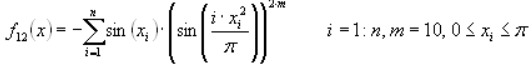
\includegraphics[width=5.54244in,height=0.7501in]{vertopal_3cc9e404d6084a9aa4179e4b559e5481/media/image4.png}

\hypertarget{metode}{%
\subsection{\texorpdfstring{3. Metode }{3. Metode }}\label{metode}}

\textbf{3.1 Reprezentare \& vecinătate.} Puncte reale calculate astfel:
prin modiicarea unei coorodonate ±$\delta$ (2·D vecini/iterație). $\delta$ este egal
cu 0.00001 , pentru o precizie de 5 zecimale.\\
\textbf{3.2 Hill Climbing (HC).}

\textbf{First Improvement} - calcularea liniara a vecinilor si alegerea
primului care are fitnesul strcit mai bun decat punctul curent\\
\textbf{Best Improvement} - calcularea tuturor vecinilor si alegerea
celui cu diferetta dintre fitnessul curent si cel al unui potential
vecin cea mai mare\\
\textbf{Worst Improvement} - calcularea tuturor vecinilor si alegerea
celui cu diferetta dintre fitnessul curent si cel al vecinului strict
mai mare ca 0 , dar minimul posibil

\textbf{3.3 Simulated Annealing (SA).} temp = temp / (1 + beta * temp) -
temperatura nouă e raportul dintre temperatura veche și~(1 + $\beta$·temp)

\textbf{3.4 Hibridizare SA+BI -- Dupa rularea alg B.I. salvez minimul
local , si aplica algorimtul S.A. din punctul respectiv.}

\textbf{3.5 Pseudocod (exemplu, varianta A)}

\texttt{function\ }\texttt{BuildBestReference}\texttt{(}\texttt{f,\ D,\ delta,\ }\texttt{num\_runs}\texttt{):}

\texttt{\ \ \ \ }\texttt{best\_ref}\texttt{\ ←\ +$\infty$}

\texttt{\ \ \ \ repeat\ }\texttt{num\_runs}\texttt{\ times:}

\texttt{\ \ \ \ \ \ \ \ result\ ←\ }\texttt{RunBestImprovement}\texttt{(}\texttt{f,\ D,\ }\texttt{delta)\ \ \ }\texttt{//\ hill\ climbing\ BI}

\texttt{\ \ \ \ \ \ \ \ if\ result\ \textless{}\ }\texttt{best\_ref}\texttt{:}

\texttt{\ \ \ \ \ \ \ \ \ \ \ \ }\texttt{best\_ref}\texttt{\ ←\ result}

\texttt{\ \ \ \ return\ }\texttt{best\_ref}

\texttt{function\ }\texttt{HybridSAwithBI}\texttt{(}\texttt{f,\ D,\ delta,\ }\texttt{initial\_temp}\texttt{,\ beta,\ }\texttt{best\_ref}\texttt{):}

\texttt{\ \ \ \ }\texttt{hc}\texttt{\ ←\ new\ }\texttt{HillClimbing}\texttt{(}\texttt{f,\ D,\ }\texttt{delta)\ \ \ }\texttt{\ \ //\ }\texttt{ctor}\texttt{\ seed}\texttt{‑}\texttt{uie}\texttt{ș}\texttt{te}\texttt{\ RNG,\ }\texttt{punct}\texttt{\ random}

\texttt{\ \ \ \ }\texttt{hc.current}\texttt{\_fitness}\texttt{\ ←\ }\texttt{best\_ref}\texttt{\ \ \ \ \ \ \ \ \ \ //\ }\texttt{pornești}\texttt{\ cu\ }\texttt{fitnessul}\texttt{\ BI}

\texttt{\ \ \ \ T\ ←\ }\texttt{initial\_temp}

\texttt{\ \ \ \ while\ }\texttt{hc.evaluations}\texttt{\ \textless{}\ }\texttt{hc.maxEvaluations}\texttt{\ and\ T\ \textgreater{}\ $\epsilon$:}

\texttt{\ \ \ \ \ \ \ \ candidate\ ←\ }\texttt{hc.GenerateRandomPoint}\texttt{()}

\texttt{\ \ \ \ \ \ \ \ }\texttt{candidate\_}\texttt{fitness}\texttt{\ ←\ f}\texttt{(candidate)}

\texttt{\ \ \ \ \ \ \ \ }\texttt{hc.evaluations}\texttt{++}

\texttt{\ \ \ \ \ \ \ \ if\ }\texttt{candidate\_fitness}\texttt{\ \textless{}\ }\texttt{hc.current}\texttt{\_fitness}\texttt{:}

\texttt{\ \ \ \ \ \ \ \ \ \ \ \ }\texttt{hc.Accept}\texttt{(candidate,\ }\texttt{candidate\_}\texttt{fitness}\texttt{)\ \ \ }\texttt{\ \ //\ }\texttt{actualizezi}\texttt{\ }\texttt{punct}\texttt{\ și\ }\texttt{componente}

\texttt{\ \ \ \ \ \ \ \ else:}

\texttt{\ \ \ \ \ \ \ \ \ \ \ \ prob\ ←\ }\texttt{exp(-(}\texttt{candidate\_fitness}\texttt{\ -\ }\texttt{hc.current}\texttt{\_fitness}\texttt{)\ /\ T)}

\texttt{\ \ \ \ \ \ \ \ \ \ \ \ if\ }\texttt{Uniform(}\texttt{0,\ 1)\ \textless{}\ prob:}

\texttt{\ \ \ \ \ \ \ \ \ \ \ \ \ \ \ \ }\texttt{hc.Accept}\texttt{(candidate,\ }\texttt{candidate\_fitness}\texttt{)}

\texttt{\ \ \ \ \ \ \ \ T\ ←\ T\ /\ (1\ +\ beta\ *\ }\texttt{T)\ \ \ }\texttt{\ \ \ \ \ \ \ //\ schema\ ta\ de\ }\texttt{răcire}\texttt{\ }\texttt{reciprocă}

\texttt{\ \ \ \ return\ }\texttt{hc.current}\texttt{\_fitness}

\texttt{//\ }\texttt{orchestrare}

\texttt{for\ each\ }\texttt{func}\texttt{\ f\ }\texttt{$\in$}\texttt{\ }\texttt{functii}\texttt{,\ }\texttt{dimensiune}\texttt{\ D:}

\texttt{\ \ \ \ }\texttt{best\_ref}\texttt{\ ←\ }\texttt{BuildBestReference}\texttt{(}\texttt{f,\ D,\ delta,\ }\texttt{num\_runs}\texttt{)}

\texttt{\ \ \ \ repeat\ }\texttt{num\_runs}\texttt{\ times:}

\texttt{\ \ \ \ \ \ \ \ }\texttt{sa\_result}\texttt{\ ←\ }\texttt{HybridSAwithBI}\texttt{(}\texttt{f,\ D,\ delta,\ }\texttt{initial\_temp}\texttt{,\ beta,\ }\texttt{best\_ref}\texttt{)}

\texttt{\ \ \ \ \ \ \ \ }\texttt{colectează}\texttt{\ }\texttt{metricile}\texttt{\ (best,\ worst,\ mean,\ $\alpha$,\ }\texttt{evaluări}\texttt{\ }\texttt{medii}\texttt{)\ }

\textbf{3.6 Cost \& echitate.} Conditia de oprire a fost cate un numar
standard constant de vecini verificati, indiferent de dimensiune. Am
implementat acest lucru printr-o inmultire care are rolul de a creste
numarul de iteratii in functie de parametrii de intrare. Am ales acest
lucru pentru ca in Dimensiunile mari, 50/100 , rezultatele erau aprox
nesemnificative , deoarece alg se oprea dupa foarte putini vecini
verificati.Parametrii functiilor de cautare au fost Functia Matematica
si Dimensiunea.

\textbf{3.7 Implementare.}

Limbaj : C++ 17

\begin{itemize}
\item
  Biblioteci:\textless algorithm\textgreater,\textless cmath\textgreater,\textless future\textgreater,\textless iomanip\textgreater,\textless iostream\textgreater,\textless limits\textgreater,\textless map\textgreater,\textless memory\textgreater,\textless numeric\textgreater,\textless random\textgreater,\textless set\textgreater,\textless sstream\textgreater,\textless stdexcept\textgreater,\textless string\textgreater,\textless thread\textgreater,\textless vector\textgreater{}
\end{itemize}

seed fixat : Seed-ul e sursa de entropie pentru generatorul
pseudo-aleator (mt19937).

Hardware : i7-13650HX si 24 GB DDR5

\hypertarget{protocol-experimental-0.51.5-pagini}{%
\subsection{4. Protocol experimental (0.5--1.5
pagini)}\label{protocol-experimental-0.51.5-pagini}}

\textbf{4.1 Configurații.} D$\in$\{5,10,30,100\}; N=50 rulari/config;
precizie output 5 zecimale.\\
\textbf{4.2 Domenii \& inițializare.} Uniform pe domeniul funcției;
multi‑start.\\
\textbf{4.3 Buget \& oprire.} Buget E per run (50,100,250)*10000 v ecini
viiztatati , obtinuti prin formula
(50,100,250)*10000*maximum(1,Dimensiune).\\
\textbf{4.4 Metrice.} ~Best,~Worst,~Mean,~Sigma~,~Evaluari
medii~,Coeficientul de Variatie și numărul total de~Rulari.

\textbf{4.6 Reproductibilitate.} Rezultatele le-am salvat intr-un fisier
cu extensia.txt sub forma de pseudo-tabela.

\hypertarget{rezultate-experimentale}{%
\subsection{\texorpdfstring{5. Rezultate experimentale
}{5. Rezultate experimentale }}\label{rezultate-experimentale}}

\textbf{5.1. Performanță finală (buget fix)} În toate cazurile,
Simulated Annealing obține o valoare medie a funcției obiectiv
semnificativ mai bună. Cea Mai Bună Soluție (Best): SA nu doar că este
mai bun în medie, dar identifică și soluții individuale (Best) mult
superioare. Performanța între Strategiile Hill Climbing: Nu există un
câștigător clar între First, Best și Worst Improvement. Performanța lor
este foarte similară în majoritatea scenariilor, sugerând că toate trei
eșuează în mod similar prin blocarea în optimi locale. De exemplu,
pentru DeJong1 (D=30, Buget Mediu), mediile sunt 267.6 (First) , 273.3
(Best) și 263.8 (Worst), valori foarte apropiate.\\
\textbf{5.3 Sensibilitate la parametri.} \textbf{Simulated Annealing
este mult mai robust.} Valorile Sigma pentru SA sunt, în mod constant,
cu unul sau mai multe ordine de mărime mai mici decât cele ale
strategiilor Hill Climbing.Pentru \textbf{Michalewicz (D=100, Buget
Mediu)}, SA are o deviație standard de doar 0.88 , în timp ce
strategiile Hill Climbing au valori între 8.9 și 13.2. Această
discrepanță uriașă indică faptul că strategiile Hill Climbing sunt
extrem de sensibile la punctul de pornire aleatoriu și se blochează în
optimi locale de calități foarte variate.

\textbf{5.4 Eficiența și Impactul Bugetului Computațional:} Simulated
Annealing (Randament Descrescător): Creșterea bugetului de evaluări
aduce beneficii minore pentru SA, sugerând că algoritmul converge
relativ repede către o soluție de înaltă calitate. Pentru Rastrigin
(D=100), trecerea de la bugetul mediu (20M evaluări, Media 1312.37) la
cel mare (40M evaluări, Media 1300.56) aduce o îmbunătățire foarte mică.
\textbf{Hill Climbing (Ineficiență):} Pentru strategiile First, Best și
Worst Improvement, creșterea bugetului computațional este
ineficientă.Pentru \textbf{Rastrigin (D=30)}, strategia Best Improvement
are o medie de 559.9 (Buget Mic) , 547.9 (Buget Mediu) și 561.4 (Buget
Mare). Nu există nicio corelație între creșterea bugetului și
îmbunătățirea soluției

\subsection{Calitatea Soluției vs. Scalabilitate}

\begin{figure}[htbp]
	\centering
	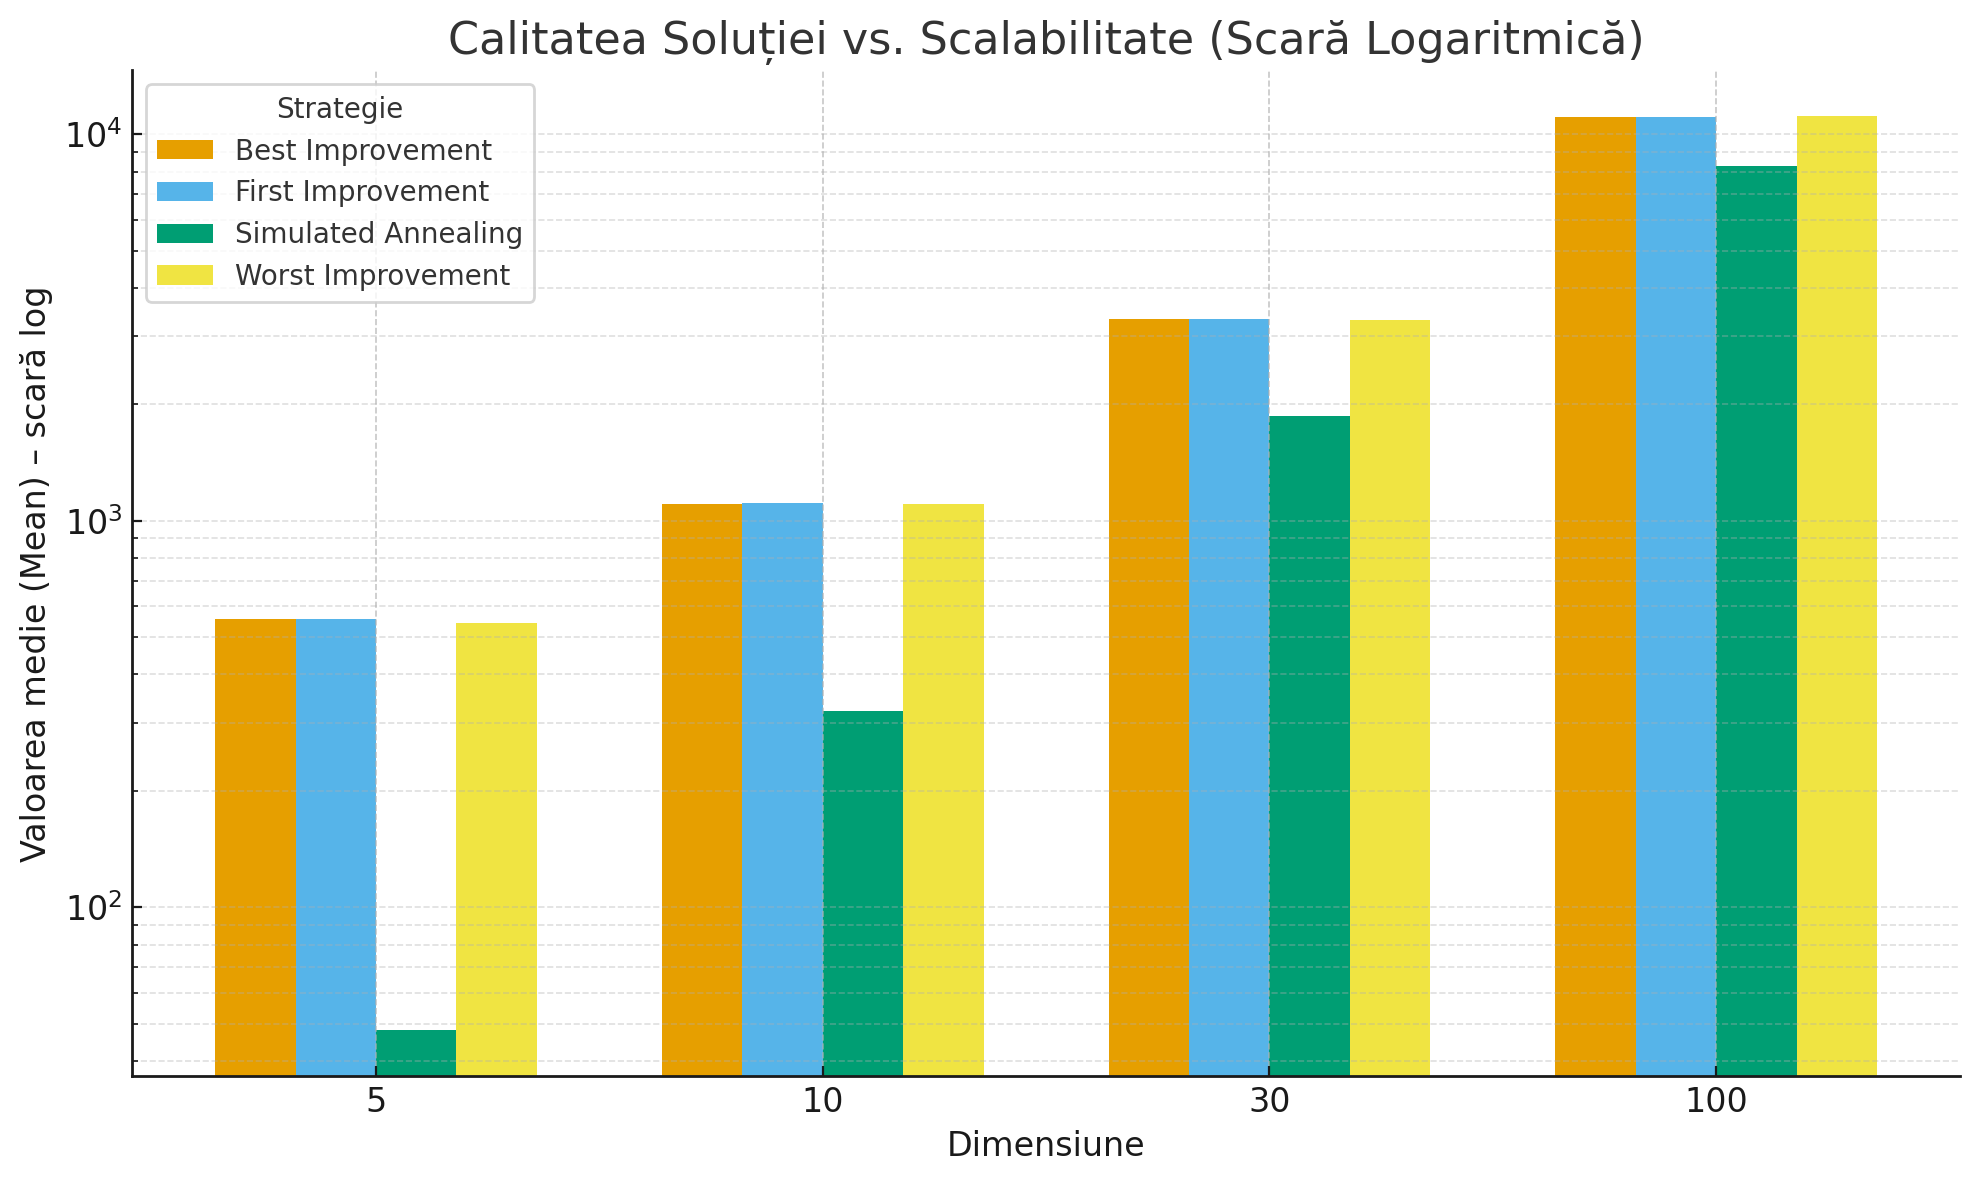
\includegraphics[width=\textwidth]{vertopal_3cc9e404d6084a9aa4179e4b559e5481/media/image5.png}
	\caption{Calitatea Soluției vs. Scalabilitate (Scară Logaritmică) }
	\label{fig:calitate-scalabilitate}
\end{figure}

\begin{figure}[htbp]
	\centering
	
	% Prima imagine
	\begin{minipage}{0.48\textwidth}
		\centering
		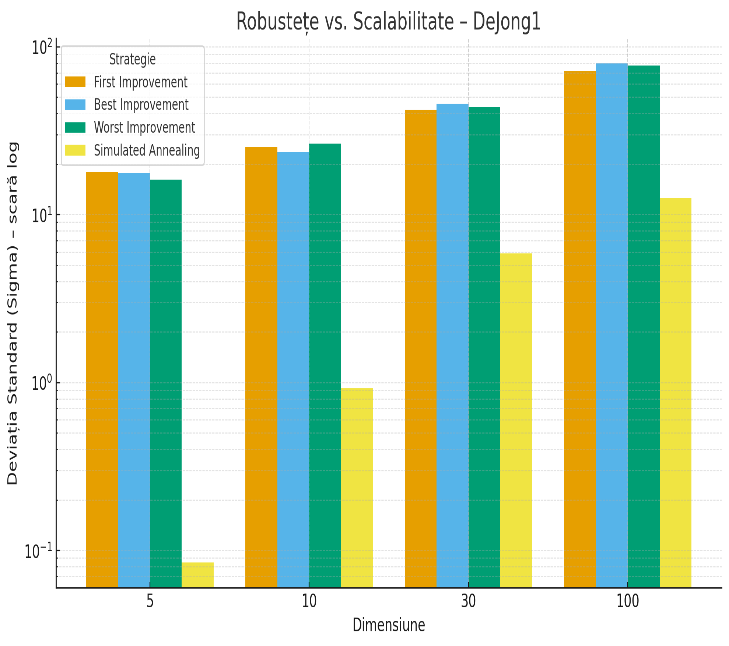
\includegraphics[width=\textwidth]{vertopal_3cc9e404d6084a9aa4179e4b559e5481/media/image6.png}
		% Puteți adăuga o sub-descriere dacă doriți
	\end{minipage}
	\hfill % Adaugă spațiu flexibil între imagini
	% A doua imagine
	\begin{minipage}{0.48\textwidth}
		\centering
		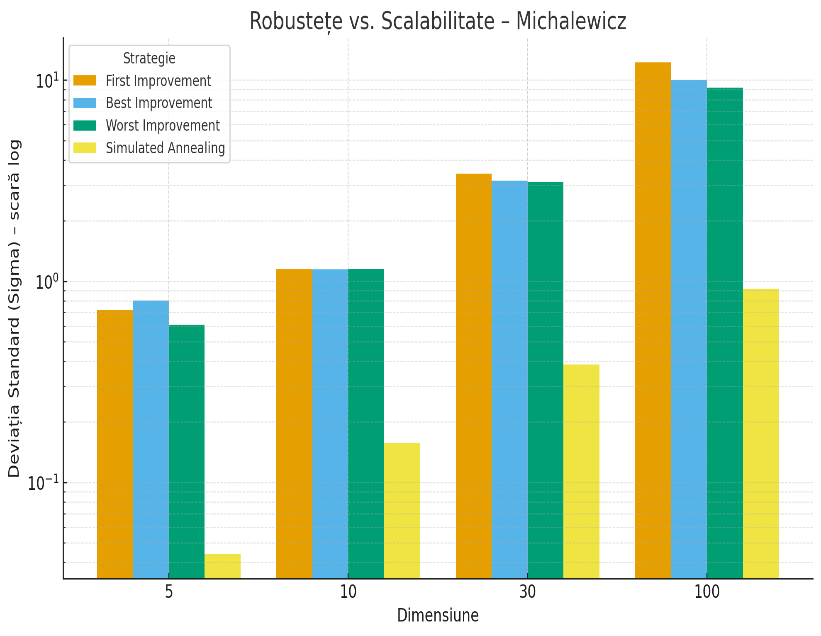
\includegraphics[width=\textwidth]{vertopal_3cc9e404d6084a9aa4179e4b559e5481/media/image7.png}
		% Puteți adăuga o sub-descriere dacă doriți
	\end{minipage}
	
	\caption{Comparația robusteții (Sigma) pentru DeJong1 (stânga) și Michalewicz (dreapta).}
	\label{fig:robustete-dejong-michal}
\end{figure}

\begin{figure}[htbp]
	\centering
	
	% Prima imagine
	\begin{minipage}{0.48\textwidth}
		\centering
		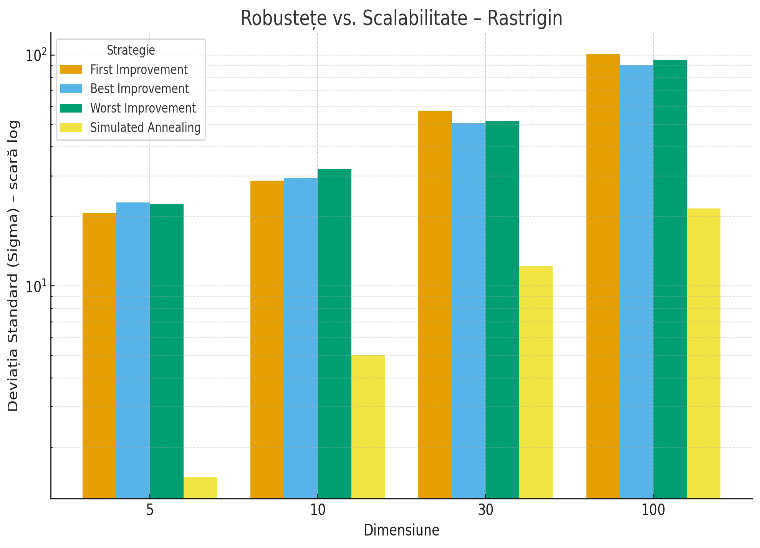
\includegraphics[width=\textwidth]{vertopal_3cc9e404d6084a9aa4179e4b559e5481/media/image8.png}
		% Puteți adăuga o sub-descriere dacă doriți
	\end{minipage}
	\hfill % Adaugă spațiu flexibil între imagini
	% A doua imagine
	\begin{minipage}{0.48\textwidth}
		\centering
		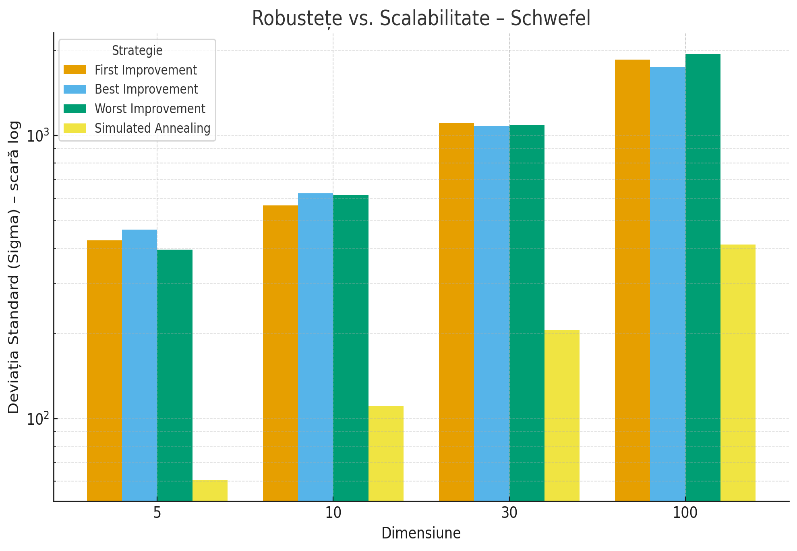
\includegraphics[width=\textwidth]{vertopal_3cc9e404d6084a9aa4179e4b559e5481/media/image9.png}
		% Puteți adăuga o sub-descriere dacă doriți
	\end{minipage}
	
	\caption{Comparația robusteții (Sigma) pentru Rastrigin (stânga) și Schwefel (dreapta).}
	\label{fig:robustete-rastrigin-schwefel}
\end{figure}

\subsection{Impactul Bugetului Computațional}

\begin{figure}[htbp]
	\centering
	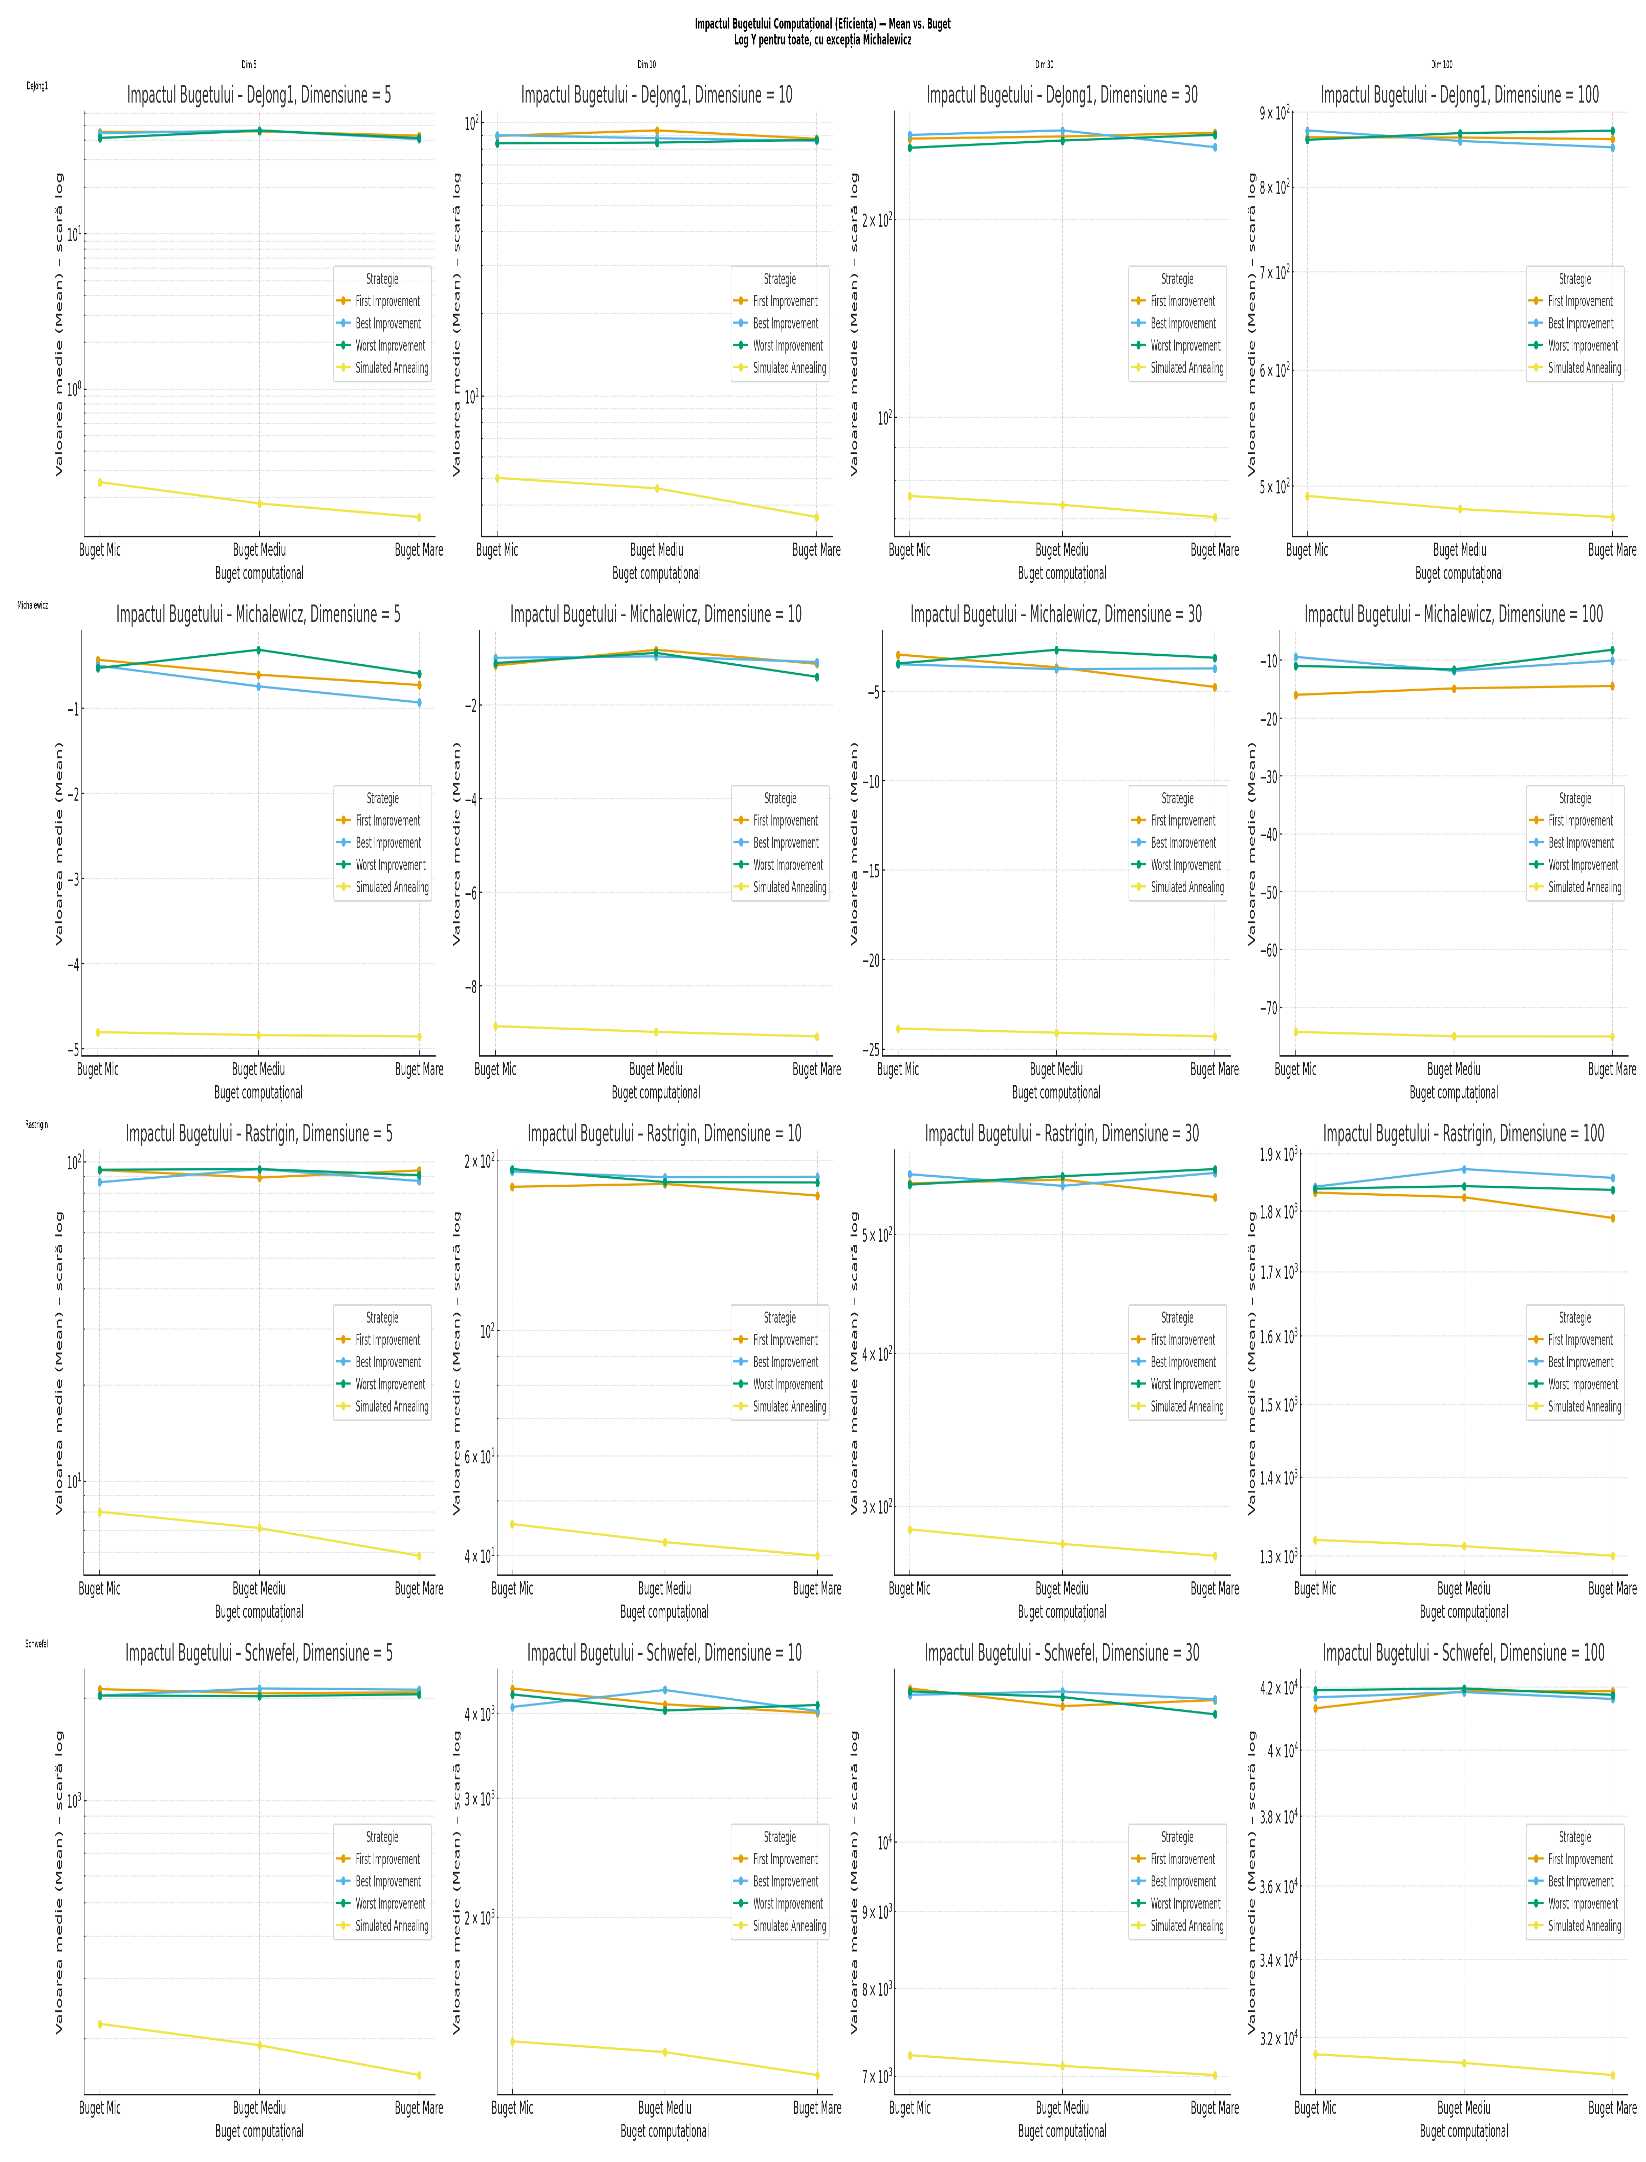
\includegraphics[width=\textwidth]{vertopal_3cc9e404d6084a9aa4179e4b559e5481/media/image10.png}
	\caption{Impactul Bugetului Computațional: Performanța medie (Mean) vs. Buget (Mic, Mediu, Mare) pentru toate funcțiile și dimensiunile. Axa Y este logaritmică, cu excepția Michalewicz.}
	\label{fig:impact-buget}
\end{figure}

\hypertarget{section}{%
\subsection{}\label{section}}

\hypertarget{interpretarea-diferenux21belor-uxeentre-metode-pe-peisaje-unimodale-vs-multimodale.}{%
\subsection{6. Interpretarea diferențelor între metode pe peisaje
unimodale vs
multimodale.}\label{interpretarea-diferenux21belor-uxeentre-metode-pe-peisaje-unimodale-vs-multimodale.}}

\hypertarget{strategiile-hill-climbing-first-best-worst-eux219ueazux103-catastrofal.-fiind-strategii-greedy-ele-urcux103-pe-primul-deal-optim-local-pe-care-uxeel-gux103sesc-ux219i-rux103muxe2n-blocate-acolo.-nu-au-niciun-mecanism-de-a-coboruxee-pentru-a-cux103uta-un-deal-mai-uxeenalt-o-soluux21bie-mai-bunux103.-acest-lucru-este-evidenux21biat-de-valorile-medii-mean-foarte-slabe-ux219i-deviaux21biile-standard-sigma-uriaux219e-care-aratux103-cux103-se-blocheazux103-uxeen-optimi-locale-diferite-la-fiecare-rulare.-simulated-annealing-sa-este-superior-cu-ordine-de-mux103rime.-datoritux103-mecanismului-sux103u-de-a-accepta-soluux21bii-mai-proaste-bazat-pe-temperaturux103-sa-poate-scux103pa-din-aceste-optimi-locale.-acest-lucru-uxeei-permite-sux103-exploreze-peisajul-global-mult-mai-eficient-ux219i-sux103-gux103seascux103-regiuni-de-soluux21bii-net-superioare-aux219a-cum-o-demonstreazux103-valorile-mean-ux219i-best-dramatic-mai-bune.}{%
\subsection{\texorpdfstring{\textbf{Strategiile Hill Climbing (First,
Best, Worst):} Eșuează catastrofal. Fiind strategii "greedy", ele urcă
pe primul "deal" (optim local) pe care îl găsesc și rămân blocate acolo.
Nu au niciun mecanism de a "coborî" pentru a căuta un deal mai înalt (o
soluție mai bună). Acest lucru este evidențiat de valorile medii (Mean)
foarte slabe și deviațiile standard (Sigma) uriașe, care arată că se
blochează în optimi locale diferite la fiecare rulare. \textbf{Simulated
Annealing (SA):} Este superior cu ordine de mărime. Datorită
mecanismului său de a accepta soluții mai proaste (bazat pe
"temperatură"), SA poate scăpa din aceste optimi locale. Acest lucru îi
permite să exploreze peisajul global mult mai eficient și să găsească
regiuni de soluții net superioare, așa cum o demonstrează valorile Mean
și Best dramatic mai bune.\\
}{Strategiile Hill Climbing (First, Best, Worst): Eșuează catastrofal. Fiind strategii "greedy", ele urcă pe primul "deal" (optim local) pe care îl găsesc și rămân blocate acolo. Nu au niciun mecanism de a "coborî" pentru a căuta un deal mai înalt (o soluție mai bună). Acest lucru este evidențiat de valorile medii (Mean) foarte slabe și deviațiile standard (Sigma) uriașe, care arată că se blochează în optimi locale diferite la fiecare rulare. Simulated Annealing (SA): Este superior cu ordine de mărime. Datorită mecanismului său de a accepta soluții mai proaste (bazat pe "temperatură"), SA poate scăpa din aceste optimi locale. Acest lucru îi permite să exploreze peisajul global mult mai eficient și să găsească regiuni de soluții net superioare, așa cum o demonstrează valorile Mean și Best dramatic mai bune. }}\label{strategiile-hill-climbing-first-best-worst-eux219ueazux103-catastrofal.-fiind-strategii-greedy-ele-urcux103-pe-primul-deal-optim-local-pe-care-uxeel-gux103sesc-ux219i-rux103muxe2n-blocate-acolo.-nu-au-niciun-mecanism-de-a-coboruxee-pentru-a-cux103uta-un-deal-mai-uxeenalt-o-soluux21bie-mai-bunux103.-acest-lucru-este-evidenux21biat-de-valorile-medii-mean-foarte-slabe-ux219i-deviaux21biile-standard-sigma-uriaux219e-care-aratux103-cux103-se-blocheazux103-uxeen-optimi-locale-diferite-la-fiecare-rulare.-simulated-annealing-sa-este-superior-cu-ordine-de-mux103rime.-datoritux103-mecanismului-sux103u-de-a-accepta-soluux21bii-mai-proaste-bazat-pe-temperaturux103-sa-poate-scux103pa-din-aceste-optimi-locale.-acest-lucru-uxeei-permite-sux103-exploreze-peisajul-global-mult-mai-eficient-ux219i-sux103-gux103seascux103-regiuni-de-soluux21bii-net-superioare-aux219a-cum-o-demonstreazux103-valorile-mean-ux219i-best-dramatic-mai-bune.}}

\hypertarget{ameninux21bux103ri-la-validitate-threats-to-validity}{%
\subsection{7. Amenințări la validitate (Threats to
validity)}\label{ameninux21bux103ri-la-validitate-threats-to-validity}}

\begin{itemize}
	\item Primul punct.
\end{itemize} \textbf{Parametrizarea Algoritmilor:} Aceasta este cea mai mare
amenințare. Simulated Annealing (SA) are parametri critici (de ex.,
schema de răcire). Dacă acești parametri au fost reglați (optimizat)
extensiv pentru aceste funcții, în timp ce strategiile Hill Climbing
(care au mai puțini parametri) au fost rulate cu setări implicite,
comparația este nedreaptă. Practic, am compara o strategie SA "reglată"
cu una Hill Climbing "nereglată".

\begin{itemize}
	\item Primul punct.
\end{itemize} \textbf{Implementarea:} Erori de implementare (bug-uri) într-una
dintre strategiile Hill Climbing ar putea să le facă să pară mai slabe
decât sunt în realitate. \begin{itemize}
	\item Primul punct.
\end{itemize} \textbf{Definiția Costului:} Costul a fost
măsurat exclusiv în număr de Evaluari medii. Această metrică ignoră
faptul că o "evaluare" SA ar putea fi mai scumpă (în timp de procesor)
decât o evaluare Hill Climbing, deoarece SA implică operații
suplimentare (generare aleatorie, calculul probabilității). O comparație
bazată pe timpul total de rulare ar putea arăta diferit.

\begin{itemize}
	\item Primul punct.
\end{itemize} \textbf{Definiția Performanței:} Performanța este măsurată ca valoarea
finală (Mean, Best) după un buget fix de evaluări. Acest lucru nu ne
spune nimic despre viteza de convergență. Este posibil ca o strategie
Hill Climbing să găsească o soluție "suficient de bună" mult mai repede,
chiar dacă soluția finală a SA este mai bună.

\hypertarget{concluzii-ux219i-lucru-viitor-1-paginux103}{%
\subsection{8. Concluzii și lucru viitor (mai mic sau egal ca 1
pagină)}\label{concluzii-ux219i-lucru-viitor-1-paginux103}}

Performanța actuală a SA se bazează pe un singur set de parametri (ex.
temperatură inițială, rată de răcire) . Nu avem garanția că aceasta este
configurația optimă.\textbf{Optimizarea Parametrilor (Meta-optimizare):}
Se propune rularea unui studiu de meta-optimizare pentru a găsi setările
optime ale SA pentru fiecare clasă de funcții.

Strategiile SA și Hill Climbing sunt, în forma lor de bază, "fără
memorie" (decizia se ia doar pe baza stării curente și a celei noi).
Adăugarea memoriei le transformă în algoritmi hibrizi, mai
puternici.\textbf{Hibridizare SA + Hill Climbing (Exploatare):} Se
propune un algoritm hibrid unde SA este folosit pentru \textbf{explorare
globală} (pentru a găsi o regiune promițătoare a spațiului), urmat de o
strategie Best Improvement pentru \textbf{exploatare locală} rapidă
(pentru a găsi rapid optimul exact din acea regiune).

\hypertarget{bibliografie}{%
\section{9. Bibliografie}\label{bibliografie}}

\begin{itemize}
\tightlist
\item
  Manual curs AG
\end{itemize}

\url{https://uaiciasi-my.sharepoint.com/:x:/g/personal/teodor_negura_student_uaic_ro/EWPZ1bTbTOJKoTZ1WFdOK7cBsGrZux6y1JyCD3iyeotO1g?e=5So9WF}

\end{document}
